% ============================================================================
%  expl4.tex -- generated by pipeline/5_results/kb_explanation.py -- do not edit by hand
%
%  One panel of the worked example for job 3031 x cv 447 (see the module docstring).
%  All labels, counts and scores are read from the ESCO v1.2.1 graph.
%
%  Compile: pdflatex expl4.tex        (needs TikZ, no extra fonts)
% ============================================================================
\documentclass[border=4pt]{standalone}
\usepackage{tikz}
\usepackage[T1]{fontenc}
\usepackage{amsmath}
\renewcommand{\familydefault}{\sfdefault}
\usetikzlibrary{arrows.meta,positioning,backgrounds,calc}

% --- palette shared with example_esco.tex ----------------------------------
\definecolor{occLeaf}{HTML}{FCE3C1}
\definecolor{skLeaf}{HTML}{CFE6F7}
\definecolor{skGrp}{HTML}{9FC9E8}
\definecolor{shared}{HTML}{E8617A}
\definecolor{faraway}{HTML}{999999}

\begin{document}
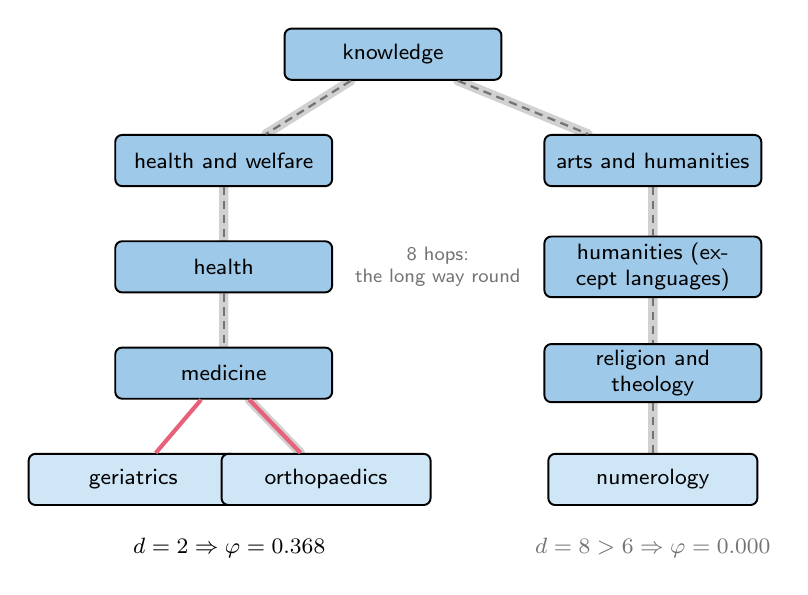
\begin{tikzpicture}[
  font=\footnotesize,
  node/.style={draw=black,line width=0.7pt,rounded corners=2.5pt,align=center,
               text width=25mm,inner sep=2.2pt,minimum height=6.5mm},
  skL/.style={node,fill=skLeaf},
  skG/.style={node,fill=skGrp,text width=26mm},
  occN/.style={node,fill=occLeaf,text width=33mm,minimum height=5mm,font=\scriptsize},
  occDead/.style={occN,fill=occLeaf!35,draw=black!45,densely dashed},
  bridge/.style={draw=shared,line width=0.9pt},
  dead/.style={draw=black!35,line width=0.7pt,densely dotted},
  broader/.style={densely dashed,draw=black!55,line width=0.8pt},
  near/.style={draw=shared,line width=1.5pt},
  detour/.style={draw=faraway!45,line width=3.4pt,line cap=round,line join=round},
  score/.style={align=center,font=\footnotesize},
  more/.style={align=center,font=\scriptsize,text=black!60},
  cross/.style={font=\normalsize,text=faraway},
  hdr/.style={font=\small\itshape,anchor=center},
]
  \node[skG] (root) at (3.30,0) {knowledge};
  \node[skG] (l0) at (1.15,-1.35) {health and welfare};
  \node[skG] (l1) at (1.15,-2.70) {health};
  \node[skG] (l2) at (1.15,-4.05) {medicine};
  \node[skG] (r0) at (6.60,-1.35) {arts and humanities};
  \node[skG] (r1) at (6.60,-2.70) {humanities (except languages)};
  \node[skG] (r2) at (6.60,-4.05) {religion and theology};
  \node[skL] (na) at (0.00,-5.40) {geriatrics};
  \node[skL] (nb) at (2.45,-5.40) {orthopaedics};
  \node[skL] (fa) at (6.60,-5.40) {numerology};
  \draw[broader] (root) -- (l0);
  \draw[broader] (root) -- (r0);
  \draw[broader] (l0) -- (l1);
  \draw[broader] (l1) -- (l2);
  \draw[broader] (r0) -- (r1);
  \draw[broader] (r1) -- (r2);
  \draw[near] (l2) -- (na);
  \draw[near] (l2) -- (nb);
  \draw[broader] (r2) -- (fa);
  \node[score,anchor=north] at (1.22,-6.02) {$d=2 \Rightarrow \varphi=0.368$};
  \node[score,anchor=north,text=black!55] at (6.60,-6.02) {$d=8 > 6 \Rightarrow \varphi=0.000$};
  \begin{scope}[on background layer]
  \draw[detour] (fa) -- (r2) -- (r1) -- (r0) -- (root) -- (l0) -- (l1) -- (l2) -- (nb);
  \node[more,text=black!55] at (3.87,-2.70) {8 hops:\\the long way round};
  \end{scope}
\end{tikzpicture}
\end{document}
